\chapter{Introducción}\label{cap1}

\section{Contexto} \label{sec:intro-contexto}
Todos los institutos de salud pública en México cuentan con proveedores que se encargan de surtir los medicamentos a sus respectivas clínicas y hospitales; el documento digital en el cual se asienta la solicitud de un medicamento es llamada orden de reposición, este documento contiene la descripción del medicamento y el lugar en donde es solicitada la entrega del mismo. En particular el Instituto para el cuál se realiza este proyecto hace llegar a los proveedores las órdenes de reposición a través de su sistema web llamado Sistema de Abastecimiento, donde el proveedor a su vez puede confirmar dentro del Sistema de Abastecimiento la recepción de las órdenes de reposición.\\
El proveedor tiene operadores dedicados a interactuar con el Sistema de Abastecimiento, las tareas que debe cumplir el operador del Sistema de Abastecimiento son: confirmar la recepción de órdenes de reposición al Sistema de Abastecimiento, obtener la información necesaria para cumplir con la entrega del medicamento (ver Figura \ref{fig:flow-proc-contestar}), y extraer las órdenes de reposición que han sido canceladas (ver Figura \ref{fig:flow-proc-verificar}), lo cual significa que el Instituto ya no requiere el medicamento especificado en la orden de reposición y de ser entregadas serán rechazadas.\\
El proveedor realiza dos tipos de procesos:
\begin{enumerate}
\item \textbf{Envío de órdenes de reposición}: un operador debe acceder al Sistema de Abastecimiento, con un usuario y contraseña previamente asignados, posteriormente debe dirigirse a la sección \textit{Contestación a Órdenes de Reposición} que es donde se muestra un listado con las órdenes de reposición emitidas por el Instituto que aún no han sido atendidas. El operador manualmente ingresa en cada orden de reposición los datos requeridos (la cantidad de unidades que enviará, fechas de fabricación y de caducidad), a esto se le conoce como responder la orden reposición.\\
En el listado de órdenes de reposición de la sección \textit{Contestación a Órdenes de Reposición} se muestra la opción de ``enviar'' cuando una orden de reposición ha sido \textit{contestada}; dicho lo anterior, el operador selecciona la opción ``enviar'' de cada una de las órdenes de reposición que ha contestado, el Sistema de Abastecimiento muestra el formato de acuse de recibo, el operador extrae los datos de interés que se muestran en el acuse y hace una impresión de la pantalla. El flujo descrito anteriormente se muestra en la Figura \ref{fig:flow-proc-contestar}.

\begin{figure}[H]
\centering

\includegraphics[scale=0.3]{flujo-proceso-contestar} 
\caption{Flujo del proceso para contestar órdenes de reposición.}
\label{fig:flow-proc-contestar}
\end{figure}

\item \textbf{Verificación de órdenes de reposición canceladas}: dado que el Instituto tiene la facultad de cancelar las órdenes aún cuando ya hayan sido enviadas, es importante para el proveedor evitar el gasto extra que implica el envío de medicamento no solicitado por el Instituto ya que implica un gasto extra el retirarlo. El operador accede al Sistema de Abastecimiento de la misma manera dirigiéndose a la sección de \textit{Consulta de Órdenes} donde el operador provee información para realizar la búsqueda (rango de fechas de emisión\footnote{Fecha en que la orden fue realizada.}, el estado de la orden como ``cancelada'') y como resultado de esta búsqueda se muestra un listado con las órdenes que cumplen con tal filtro, así el operador copia la lista en un documento local en su equipo personal, para posteriormente realizar de forma manual tal filtro, con el fin de obtener las órdenes de reposición que han sido canceladas de las cuales no se tenía conocimiento. En la Figura \ref{fig:flow-proc-verificar} se muestra el proceso para verificar las órdenes de reposición canceladas.
\begin{figure}[H]
\centering
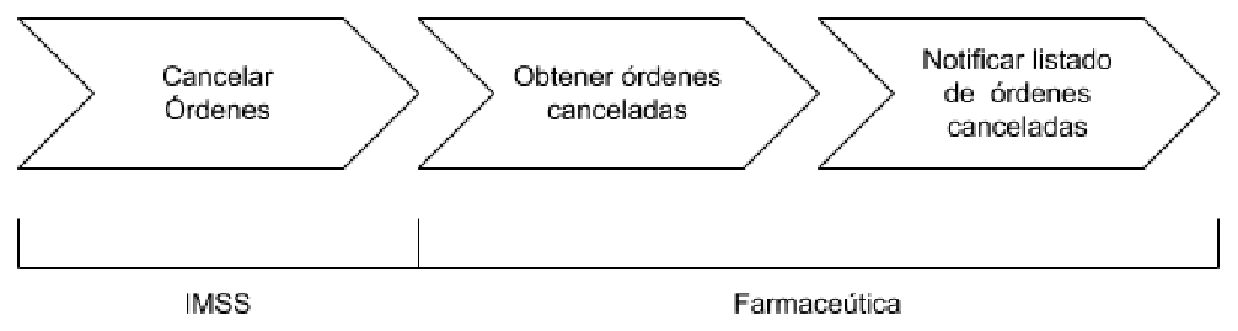
\includegraphics[scale=0.3]{flujo-proceso-verificar} 
\caption{Flujo del proceso para verificar órdenes de reposición canceladas.}
\label{fig:flow-proc-verificar}
\end{figure}
\end{enumerate}

El proveedor\footnote{Quien requiere automatizar la interacción con el Sistema de Abastecimiento para el envío de las órdenes de reposición y la verificación de órdenes canceladas.} representa a la compañía farmacéutica, por lo que en este documento nos referiremos al proveedor como a la compañía farmacéutica, o simplemente farmacéutica de manera indistinta. Los requerimientos funcionales del proveedor son la automatización de las tareas de interacción del operador con el Sistema de Abastecimiento y la elaboración de reportes estadísticos sobre las órdenes de reposición procesadas durante la automatización.

\section{Objetivos}
\subsection{Objetivo principal}\label{sec:objetivo-principal}
Realizar un sistema de cómputo, de ahora en adelante llamado \textbf{AutoSA}, que reduzca el tiempo para contestar las órdenes de reposición, ayudando a mejorar, a su vez el tiempo que toma a la farmacéutica atender las órdenes de reposición, esto implica una reducción en tiempo desde que la orden es publicada en el Sistema de Abastecimiento hasta que el medicamento es entregado físicamente al Instituto.\\
El uso del sistema AutoSA evita el envío de medicamentos que ya no son solicitados, minimizando el consumo de recursos innecesarios, así como el tiempo que toma retirar del Instituto tales medicamentos cancelados.\\
Dado que la farmacéutica atiende las órdenes de reposición del Instituto en el doble de tiempo que su competencia, en particular contestar estas órdenes en el Sistema de Abastecimiento requiere de tres personas dedicadas exclusivamente a ello, y un día completo el terminar esta parte del proceso. La solución propuesta para acelerar la respuesta y verificación de órdenes de reposición del Sistema de Abastecimiento se encuentra programado por agentes\footnote{Agente dentro de este trabajo se refiere a las rutinas que automatizan los procesos realizados por los operadores del Sistema de Abastecimiento.}, cada agente se dedica a emular las acciones del operador de la farmacéutica, el cual es el responsable de contestar o verificar las órdenes de reposición. El sistema AutoSA cuenta con una base de datos donde se almacenen los datos capturados por lo agentes durante la respuesta de órdenes, y una interfaz gráfica donde los trabajadores de la farmacéutica puedan realizar tareas de administración como son: la búsqueda, edición de órdenes de reposición y generación de reportes de las órdenes atendidas por los agentes.
\subsection{Objetivos secundarios}\label{sec:objetivos-secundarios}
\begin{enumerate}
\item Reducción del error humano en relación a la manipulación de la información.
\item Ahorro de recursos en la entrega de medicamentos no solicitados.
\item Reducción de tiempo en cuanto a la respuesta de órdenes de reposición.
\item Consistencia en los datos respecto a la generación de reportes estadísticos sobre las órdenes de reposición procesadas.
\end{enumerate}
Por lo anterior los afiliados del Instituto se verán beneficiados, pues los medicamentos estarán disponibles con mayor frecuencia en las clínicas y hospitales.

\section{Descripción general de trabajo}\label{sec:desc-general}
La farmacéutica dedica diariamente un equipo constituido por tres personas durante toda la jornada laboral, dependiendo del volumen de órdenes de reposición emitidas por el Instituto se puede agregar una persona más al equipo, para completar las tareas de envío de órdenes de reposición y verificar las órdenes de reposición canceladas dentro del Sistema de Abastecimiento.\\
A través del proyecto de automatización se pretenden optimizar los siguientes puntos:
\begin{itemize}
\item Reducción del esfuerzo de recursos humanos.
\item Eliminar los errores de captura.
\item Reducción del tiempo dedicado al envío de las órdenes de reposición.
\item Detectar con rapidez las órdenes de reposición que hayan sido canceladas.
\end{itemize}
La necesidad de automatización de los procesos (ver Figuras \ref{fig:flow-proc-contestar} y \ref{fig:flow-proc-verificar}) antes mencionados pronostican una reducción de costos por devolución de medicamento no solicitado para el cliente y también la disminución de pérdidas en las ventas por solicitudes no atendidas en los rangos de tiempo acordados con el comprador. Dado lo anterior, se plantea un proyecto de software que cubra las necesidades de automatización y pueda ser administrado por usuarios no especializados en computación.\\
Para resolver el desarrollo del proyecto, el sistema AutoSA se divide en módulos con funcionalidades específicas que se muestran a continuación:
\begin{enumerate}
\item \textbf{Automatización de interacción con el Sistema de Abastecimiento}. La automatización de la interacción con el Sistema de Abastecimiento consiste en replicar los pasos que sigue una persona de la farmacéutica (operador) encargada de llenar y extraer información de las órdenes de reposición del Sistema de Abastecimiento, es decir, listar los pasos que sigue el operador cuando contesta las órdenes de reposición, describir las reglas de negocio necesarios para llenar los formularios que presenta el Sistema de Abastecimiento al responder una orden de reposición. Por último se identifican las fuentes de los datos que se ocupan para llenar tales formularios y se define la forma de almacenamiento de la información necesaria de cada formulario.
\item \textbf{Generación de reportes}. La generación de reportes consiste en plasmar la información obtenida de las órdenes de reposición contestadas en el módulo anterior. La farmacéutica tiene ya una plantilla que se utiliza para pasar los pedidos a otras áreas, con el fin de continuar la atención de las órdenes de reposición; además de obtener estadísticas relacionadas con la cantidad de órdenes de reposición atendidas y canceladas.
\item \textbf{Interfaz de usuario}. La interfaz de usuario se refiere a la aplicación que muestra una interfaz gráfica en la cual los operadores de la farmacéutica pueden solicitar la generación de reportes; hacer consultas y modificaciones a las órdenes de reposición atendidas por el primer módulo.
\end{enumerate}

\subsection{Arquitectura de la solución}
Una definición de arquitectura de software es dada por Bourque\cite{SWEBOOK}:
\begin{quote}
El conjunto de estructuras necesarias para la comprensión de un sistema en el cual se comprometen elementos de software, relaciones entre ellos y sus propiedades.
\end{quote}
Esta definición expone que los requerimientos del cliente se traducen en especificaciones técnicas para los desarrolladores. Aplicando la definición anterior al presente proyecto donde tenemos los siguientes componentes (ver Figura \ref{fig:dia-arq-comp}):
\begin{figure}[h]
\centering
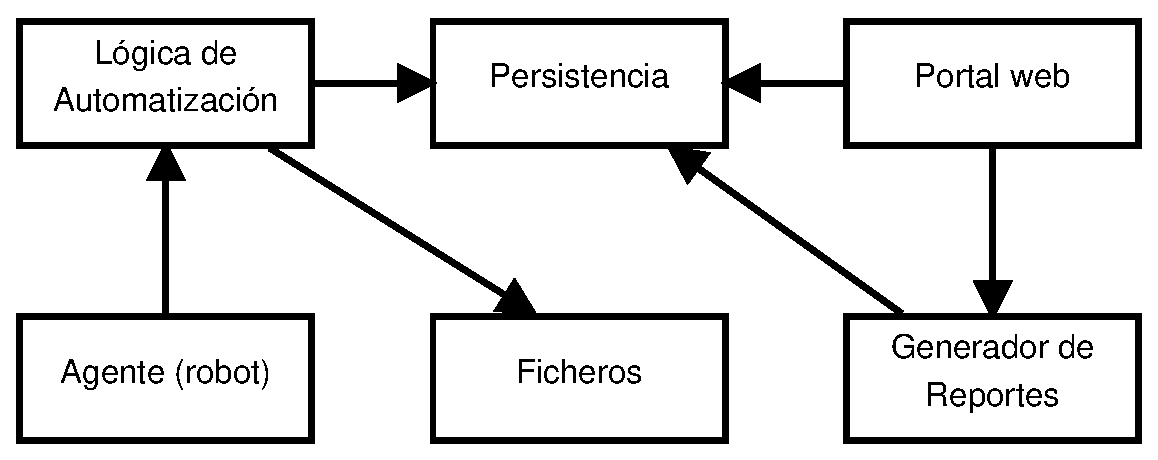
\includegraphics[scale=0.45]{dia-arq-comp} 
\caption{Módulos de la arquitectura.}
\label{fig:dia-arq-comp}
\end{figure}

\begin{itemize}
\item \textbf{Agente (robot)}. Interactúa directamente con el Sistema de Abastecimiento, es el componente que automatiza las acciones de los operadores humanos de la farmacéutica.
\item \textbf{Lógica de negocio}. Son bibliotecas y rutinas que se encargan de prestar los servicios necesarios al agente para su funcionamiento, permite comunicación con la base de datos, guarda las capturas de pantalla en el Sistema de Archivos y provee la configuración de inicio al agente.
\item \textbf{Base de datos}. Es el componente que se encarga de llevar la persistencia de los datos obtenidos durante la respuesta a las órdenes de reposición.
\item \textbf{Sistema de archivos}. En el Sistema de Archivos se almacenan las capturas de pantalla al momento de enviar la respuesta de cada orden de reposición.
\item \textbf{Generador de reportes}. Este módulo está encargado de la generación de reportes tales como: órdenes de reposición atendidas, canceladas y formatos de órdenes de reposición enviadas.
\item \textbf{Portal web}. Portal mediante el cual los usuarios pueden hacer correcciones a los datos obtenidos de las órdenes de reposición, reimprimir el formato de envío de la orden de reposición  y descargar los reportes generados por el módulo generador de reportes.
\end{itemize}

\subsection{Metodología utilizada}
El proyecto será abordado con la metodología Scrum, el cual es un marco de trabajo para desarrollar, entregar y mantener productos complejos. Scrum consiste en un conjunto de roles, eventos, artefactos y reglas que los ligan. Scrum da un enfoque adaptivo mientras promueve la entrega continua de soluciones, y divide el desarrollo en ventanas de tiempo llamadas sprint\cite{scrum}.\\
La liberación del sistema AutoSA consiste en el despliegue del total de los módulos en el ambiente productivo provisto por la farmacéutica, dando como resultado los siguientes productos:
\begin{itemize}
\item Rutinas para la generación de objetos en base de datos.
\item Rutinas para la creación de la estructura de directorios en el Sistema de Archivos.
\item Archivos de configuración propio de cada módulo.
\item Herramienta de automatización y del automatización.
\item Bibliotecas del portal web.
\item Manual de instalación y de usuario.
\item Capacitación a usuarios finales.
\end{itemize}
 
\section{Resumen}
El Instituto de Salud mediante su Sistema de Abastecimiento realiza las órdenes de reposición de medicamentos a las farmacéuticas, estas últimas invierten veinticuatro horas hombre por día para lograr contestar todas las órdenes de reposición, si se pudiera reducir el tiempo en que se atienden significaría un aumento en la velocidad de respuesta de la farmacéutica para entregar los medicamentos a centros de salud del Instituto, motivo por el cual le interesa automatizar esta parte. El sistema AutoSA que se propone en este documento da solución mediante dos subsistemas: uno que automatiza los procedimientos de interacción con el Sistema de Abastecimiento y otro que permite a los operadores de la farmacéutica generar reportes y acceder a datos de las órdenes de reposición atendidas.